
\section{Result and discussions}
To get realistic data on how the system would perform in action, a stand to showcase the product was held in the cafeteria of the University of Agder. A picture of the stand is shown in figure \ref{fig:bestExample}


\begin{figure}[h]
    \centering
    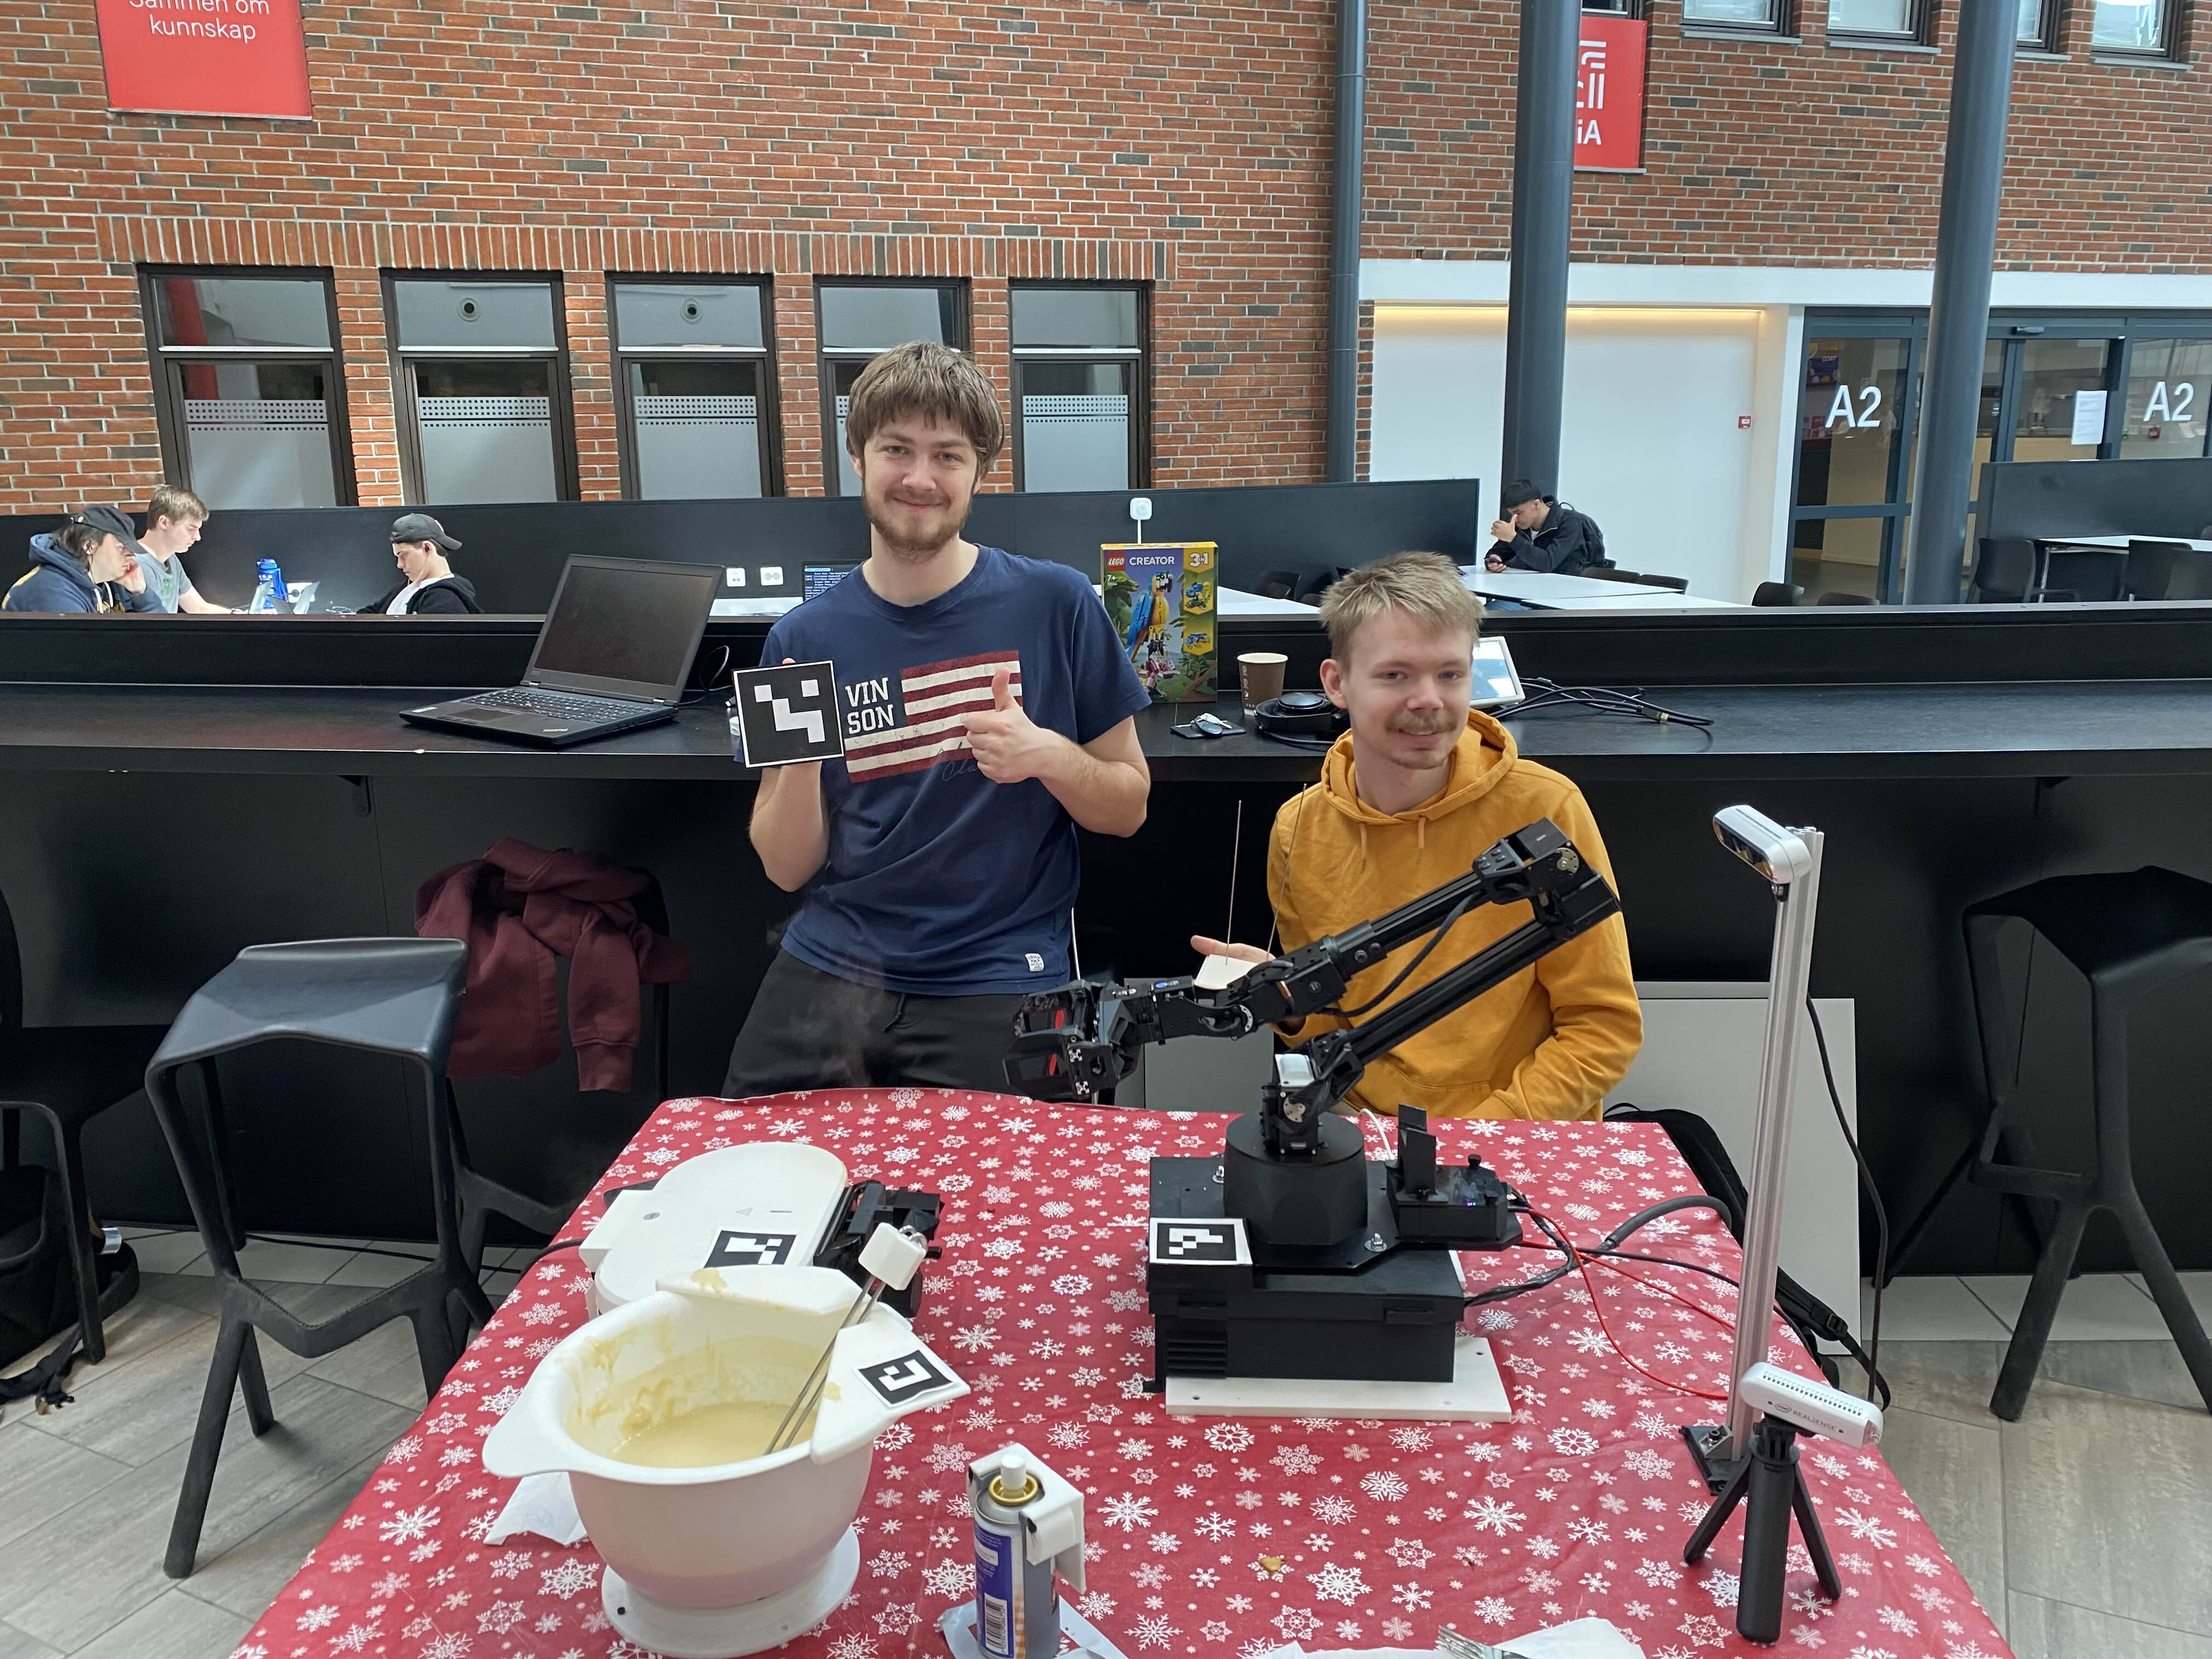
\includegraphics[width= 0.999\linewidth]{figures/waffle_stand.png}
    \caption{Waffle stand in action}
    \label{fig:bestExample}
\end{figure}
The stand was a success, both in terms of technical performance and marketing potential. On the technical side, the robot achieved a 100\% success rate, at a total cooking voume of one batch o' batter. On the marketing side, the stand drew a crowd estimated at 15 people looking onto the robot during its startup phase, settling down to an average of 5 onlookers during the first two hours of operation. Onlookers were primarily interested in the parts of the process where the robot prepared the waffle for cooking, and the final serving of the waffles. The marker tracking entertainment mode that was used did not raise interest in the stand significantly. The HMI was developed but not fully integrated to the system at the time, so a proof of concept of the HMI was shown. The feedback of the HMI was fortunately positive, the spectators were able to see operator page on the HMI.

The system was significantly more reliable when the robot used its fallback mode of predetermined positions. The camera assisted mode was only capable of performing small sets of movement reliably. Large-scale camera integrated tests led to edge cases that were not accounted for, and therefore tended towards failure. When motion sequences were tested induvidually, observed reliability increased and movements tended towards successful execution. 


